\documentclass[a4paper]{article}
\usepackage{amsmath, amssymb, graphicx}
\usepackage{url, hyperref}
\hypersetup{colorlinks=true, urlcolor=cyan}


\begin{document}
\begin{center} \Large Deep learning in audio, homework 5, anti-spoofing \end{center}
\hspace*\fill Alexey Slizkov\\
\hspace*\fill 17.12.2023\\
\vspace{25pt}



\section{The mode}

RawNet2 with SincConv of type S1.



\section{A lot of time spent on...}

Debugging a very stupid bug. Loss was good, but EER score was awful. I was trying to find the bug in my implementation of the model for a long time, but to no avail. I've gone over many permutations of batchnorms and skip-connections and so on, minor details which didn't play a role, which agrees with my intuition, as well as details of SincConv, such as whether we mirror or not, what are the gaps (0 or 30/50), etc. It turned out, the bug was not in the model, but in the computation of EER: the provided function \verb|calculate_eer| computes EER from two arguments, I thought the predictions of bonafide on real bonafide, and the predictions of spoof on real spoof. It turned out it was expecting the predictions of bonafide on real bonafide, and the prediction of \textit{bonafide} on real spoof.

Although this project contains approximately one hundred runs, most of them were debugging; the following ones are important.



\section{Main run}

Link: \url{https://wandb.ai/elexunix/as_project/runs/8rmrzw80/overview?workspace=user-elexunix}.

Uses Peh's hyperparameters and other recommendations.

The model has 16578658 parameters. Its checkpoint can be found at\\ \verb|default-test-model/main_model_best.pth|
To train, run \verb|python3 train.py|, to test, run \verb|python3 test.py|.

Test EER score of the model: 0.04446.

\begin{center} 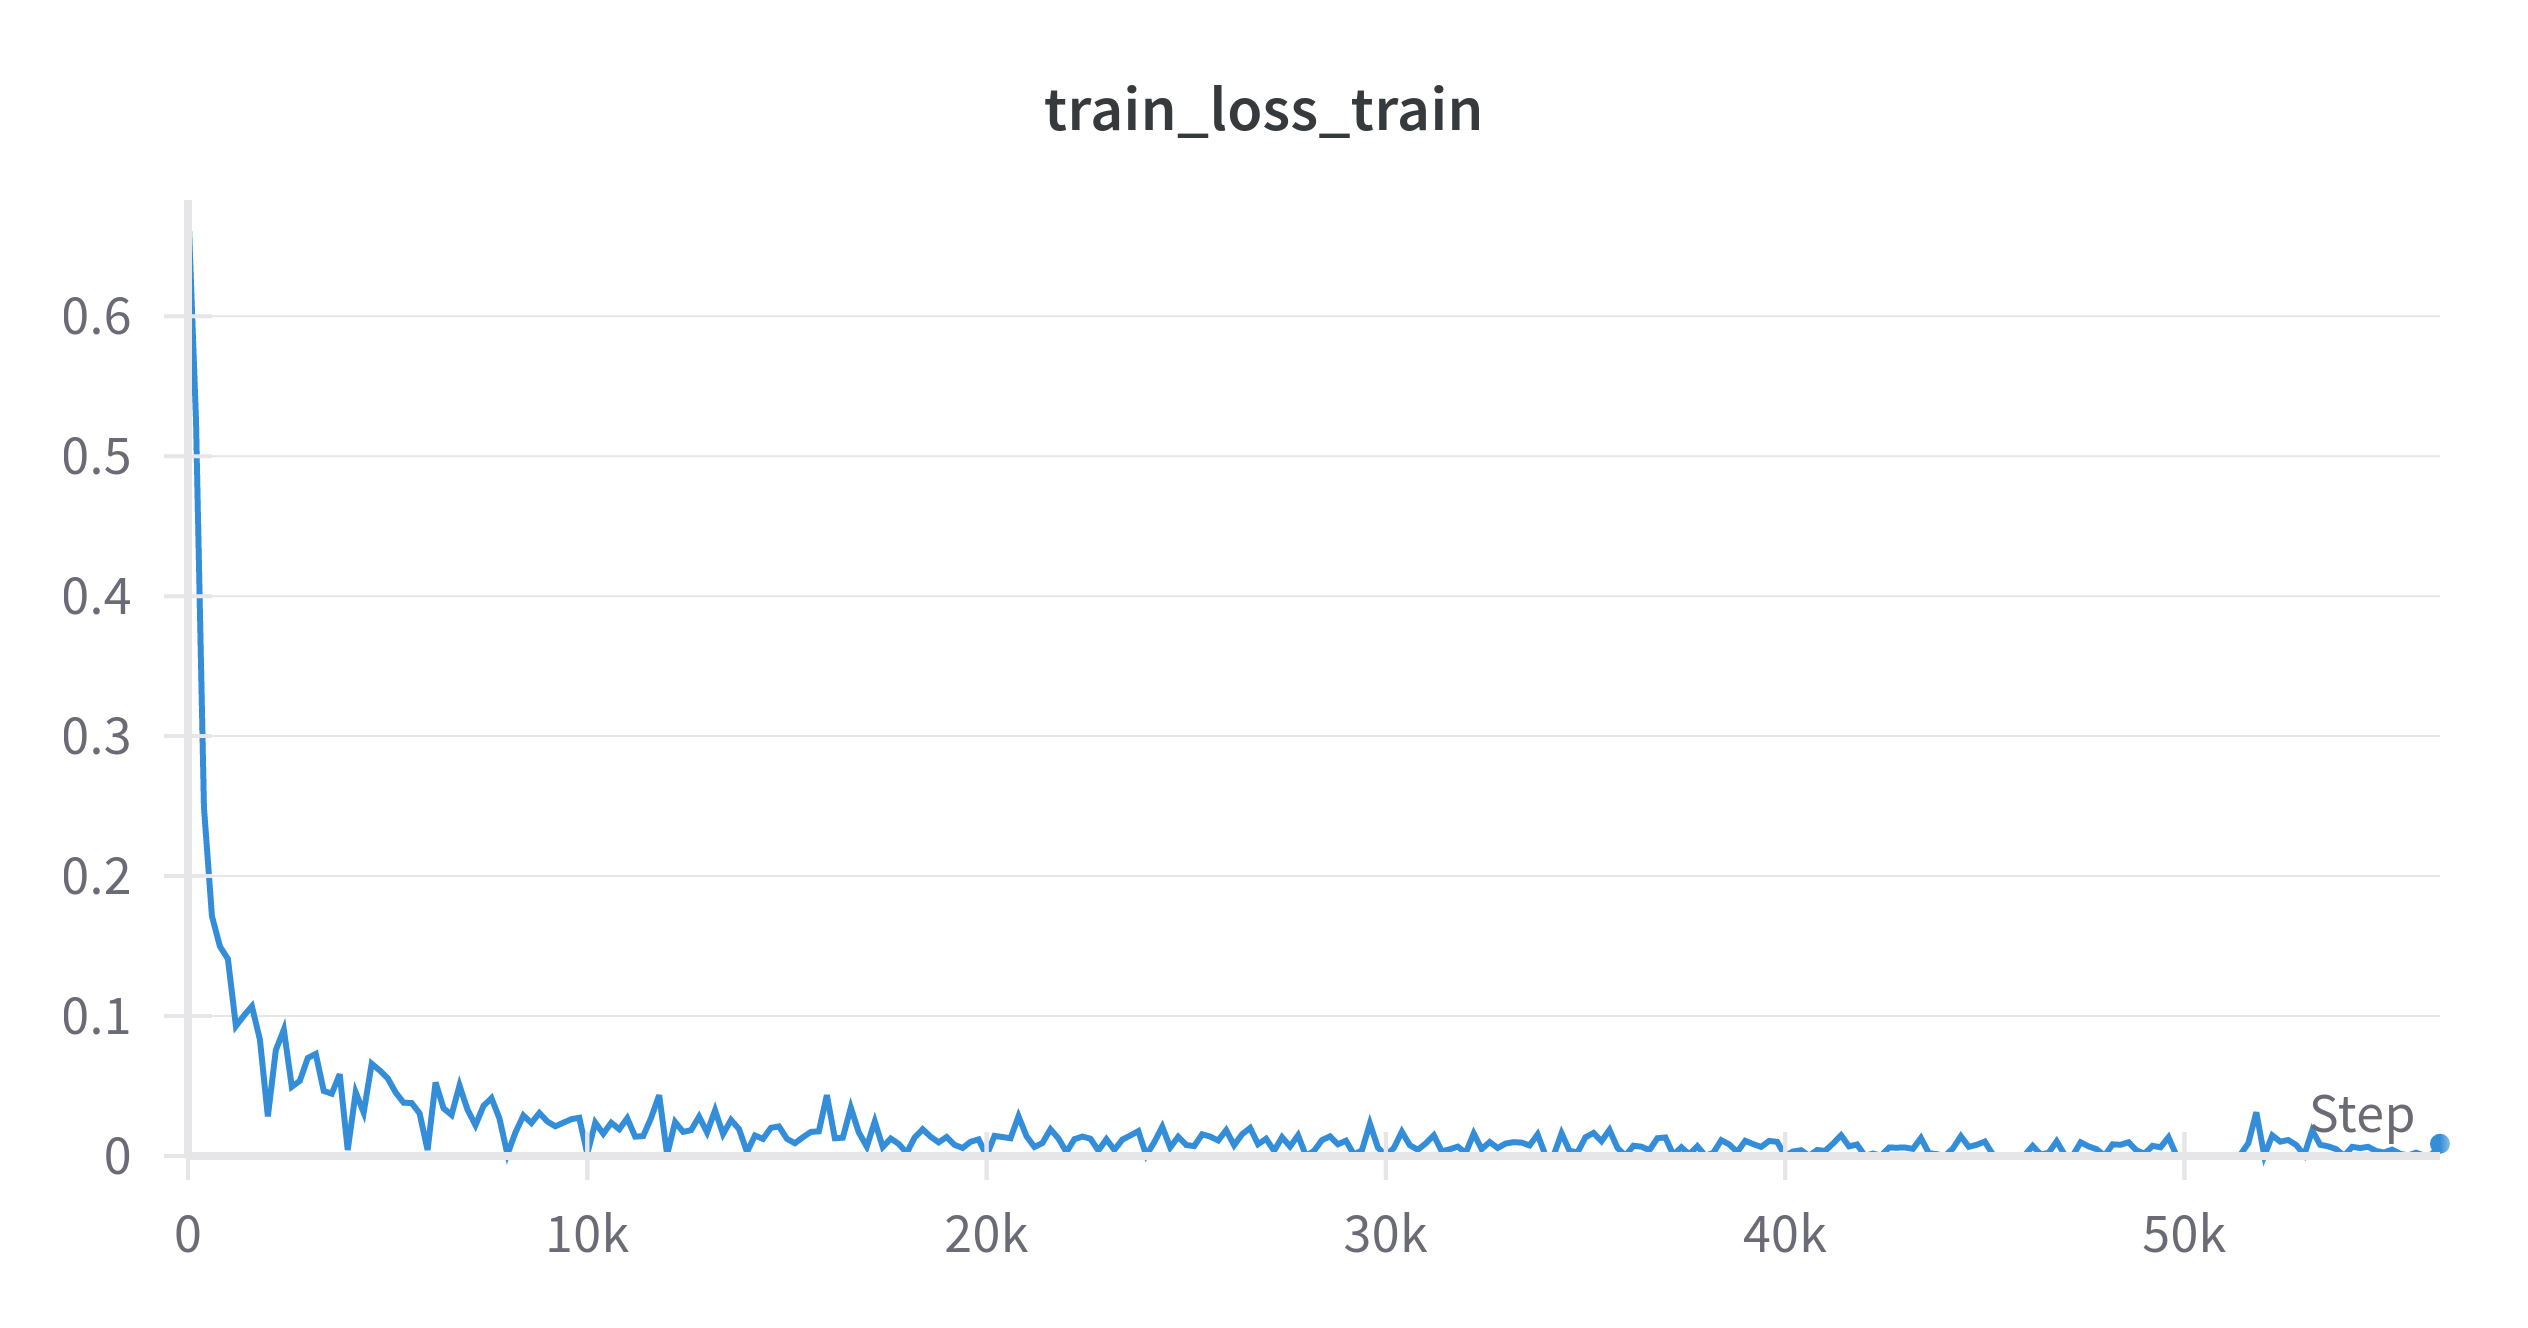
\includegraphics[width=400pt]{train-loss.png} \end{center}

\begin{center} 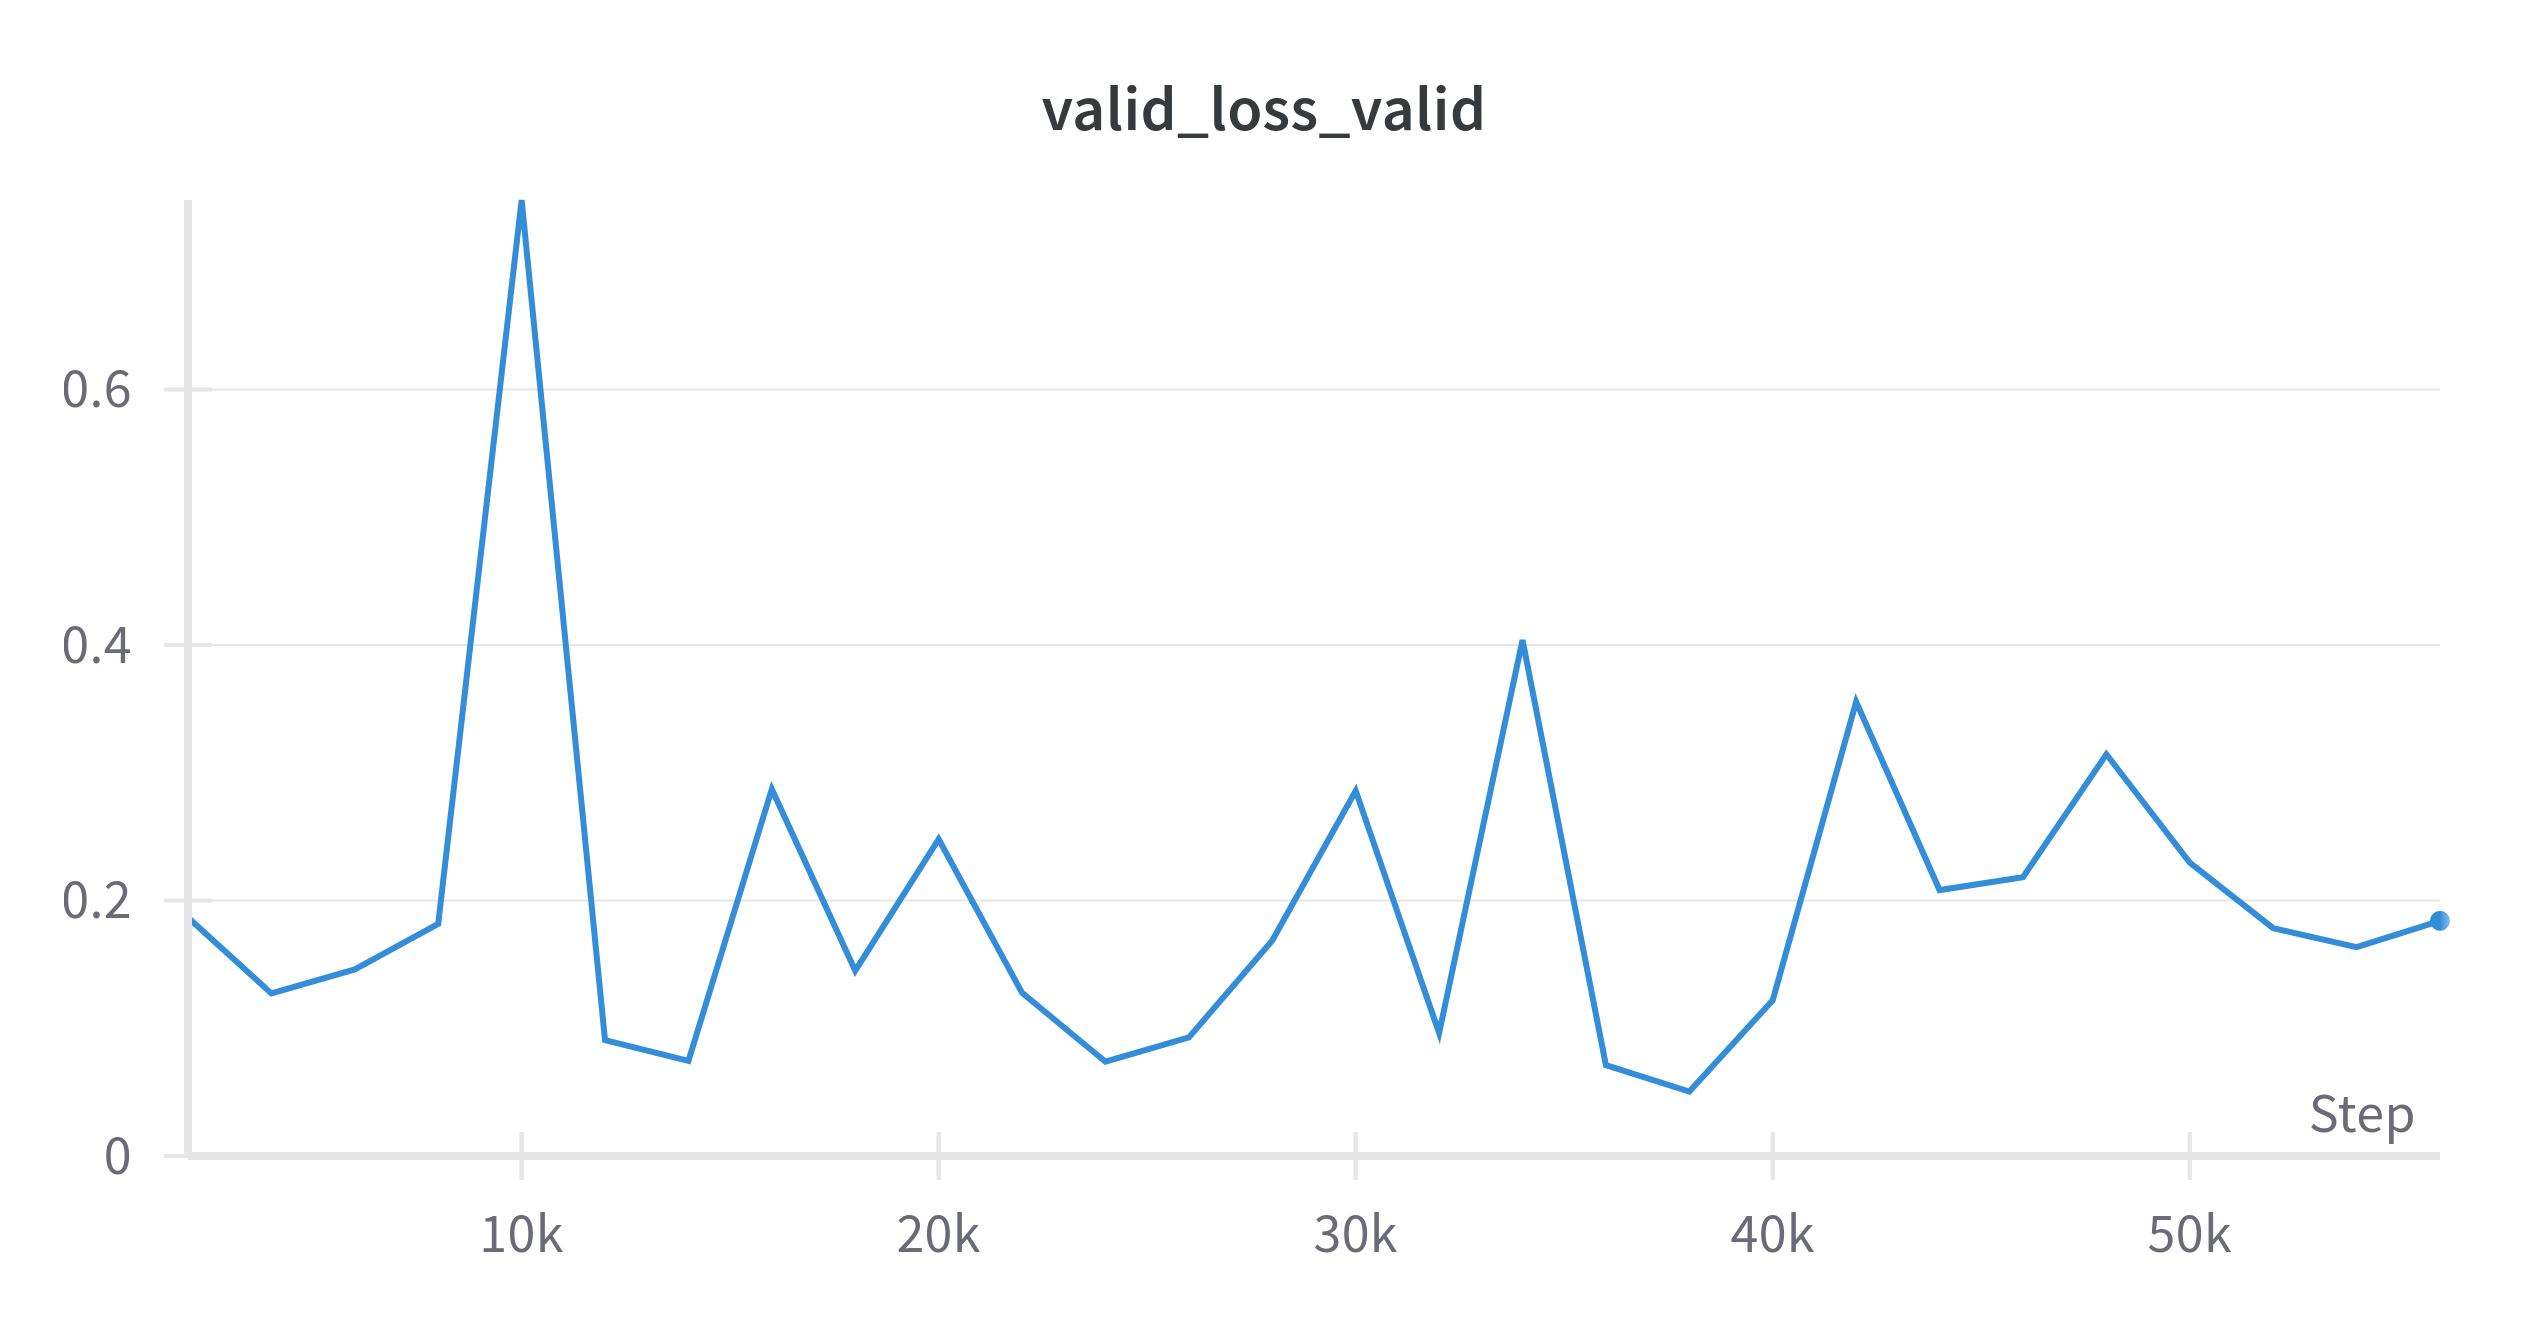
\includegraphics[width=400pt]{valid-loss.png} \end{center}

Sorry for the last word of title, it should be ignored, but hard to correct now since this is a picture from wandb.

\begin{center} 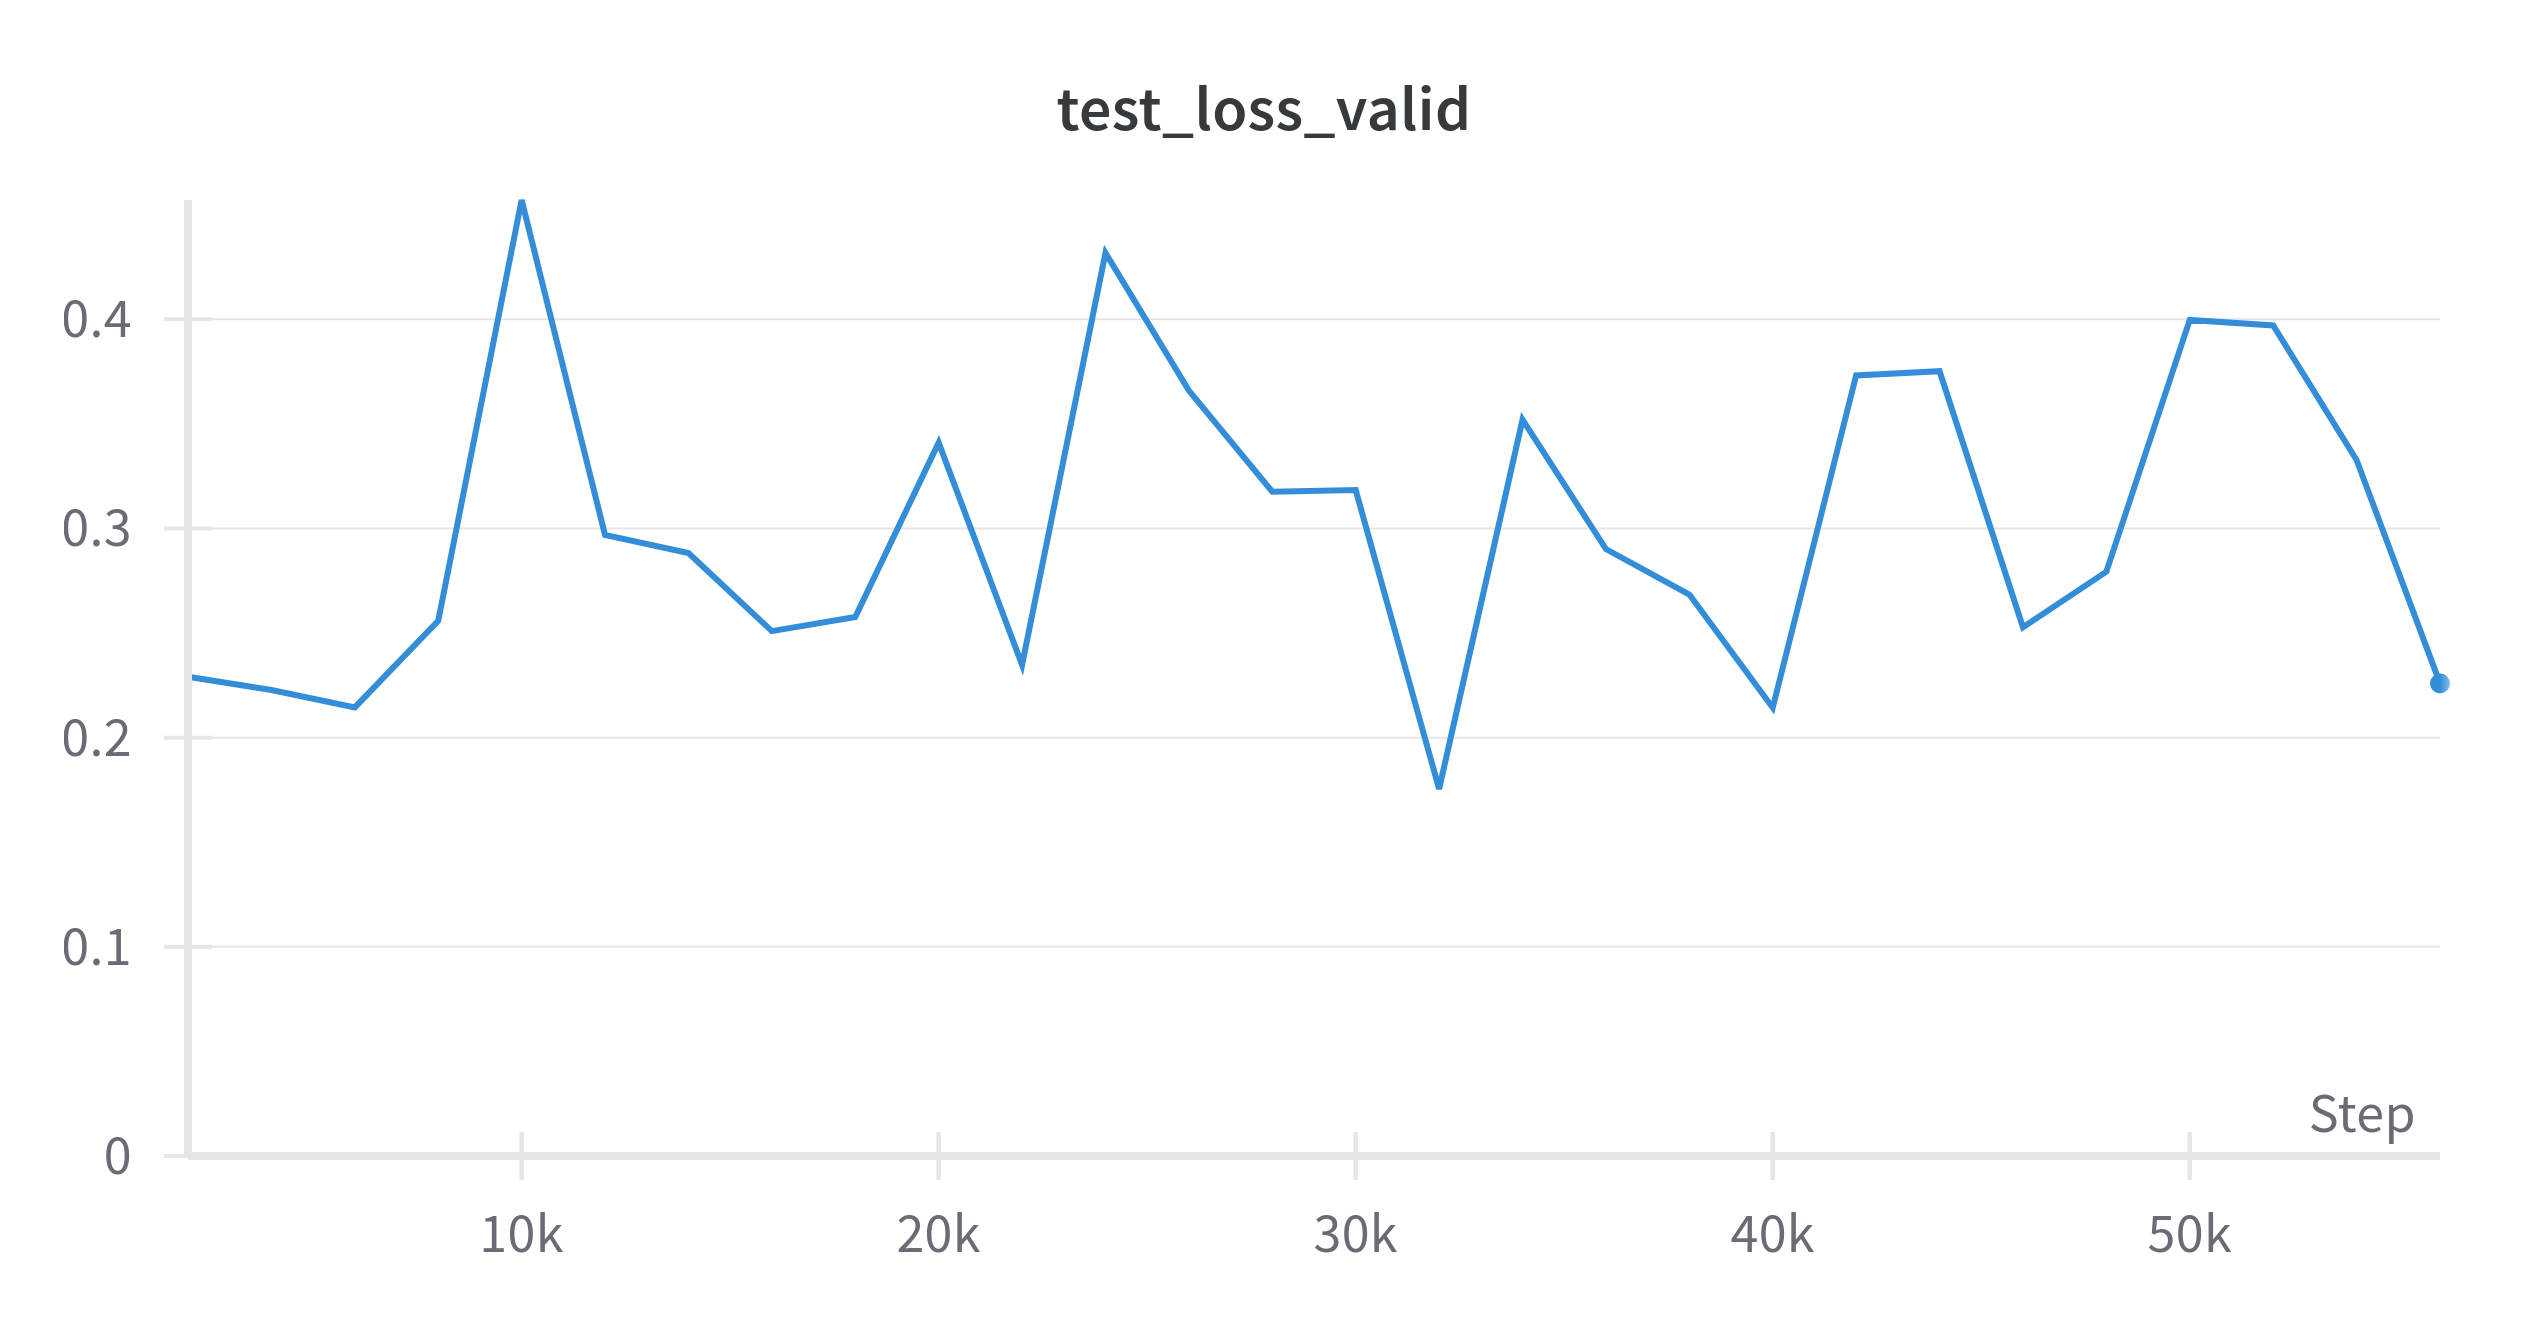
\includegraphics[width=400pt]{test-loss.png} \end{center}

\begin{center} 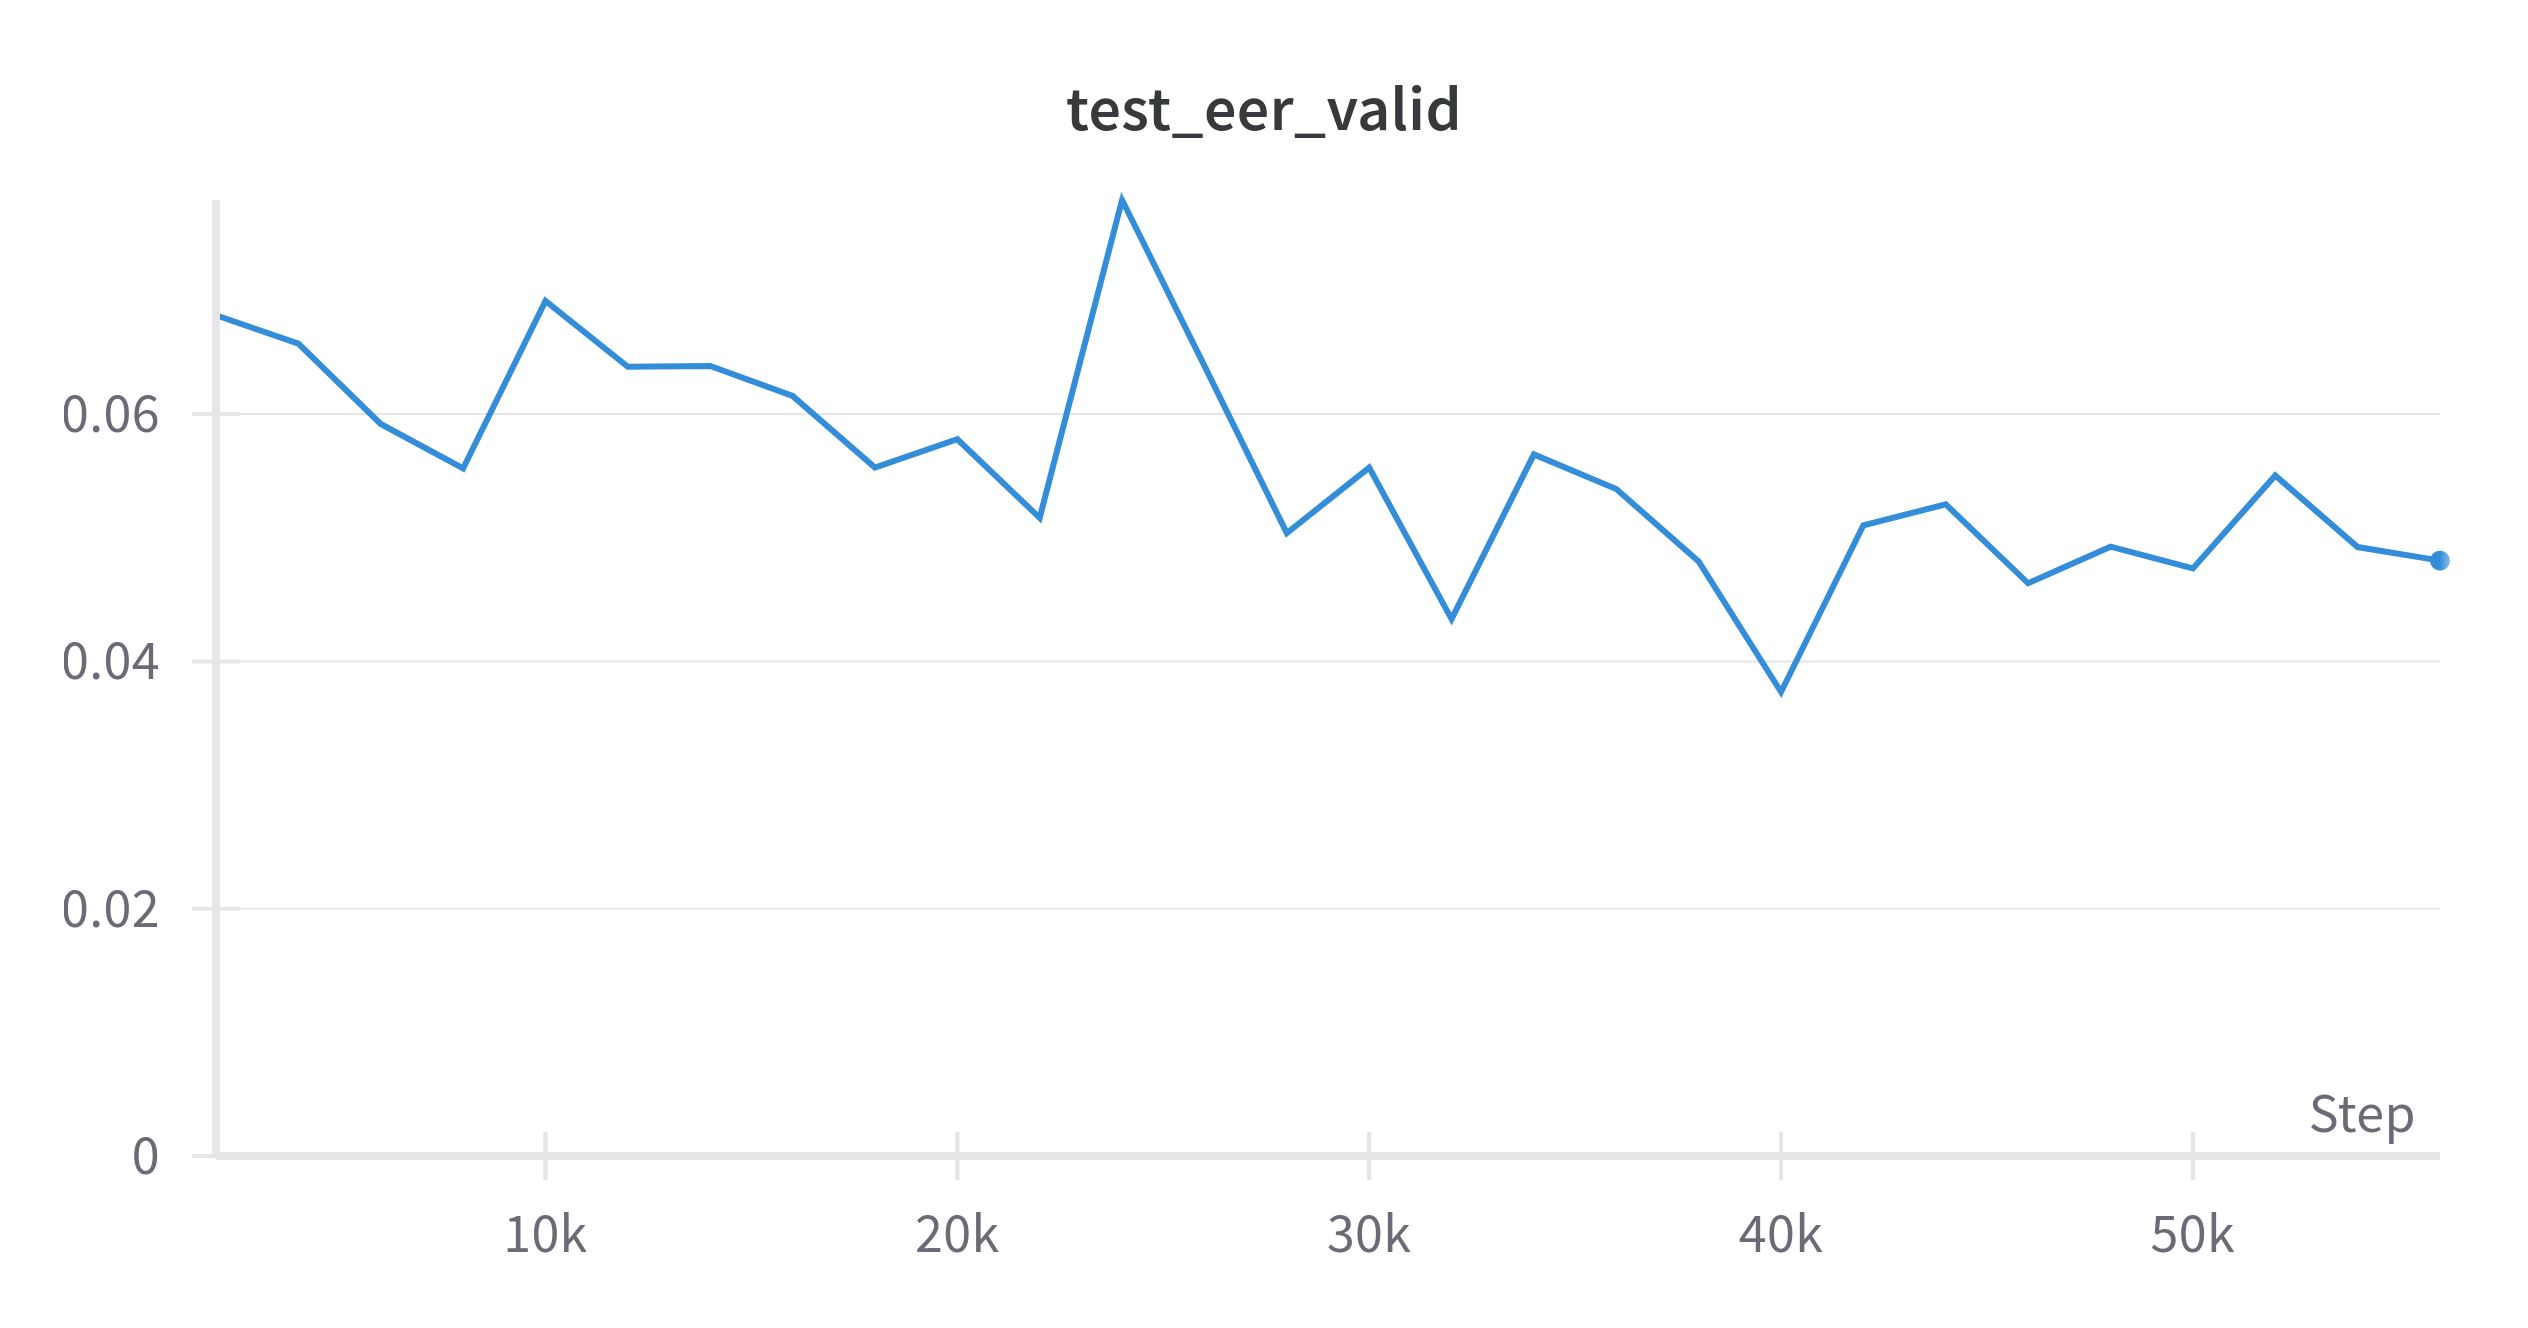
\includegraphics[width=400pt]{test-eer.png} \end{center}

\begin{center} 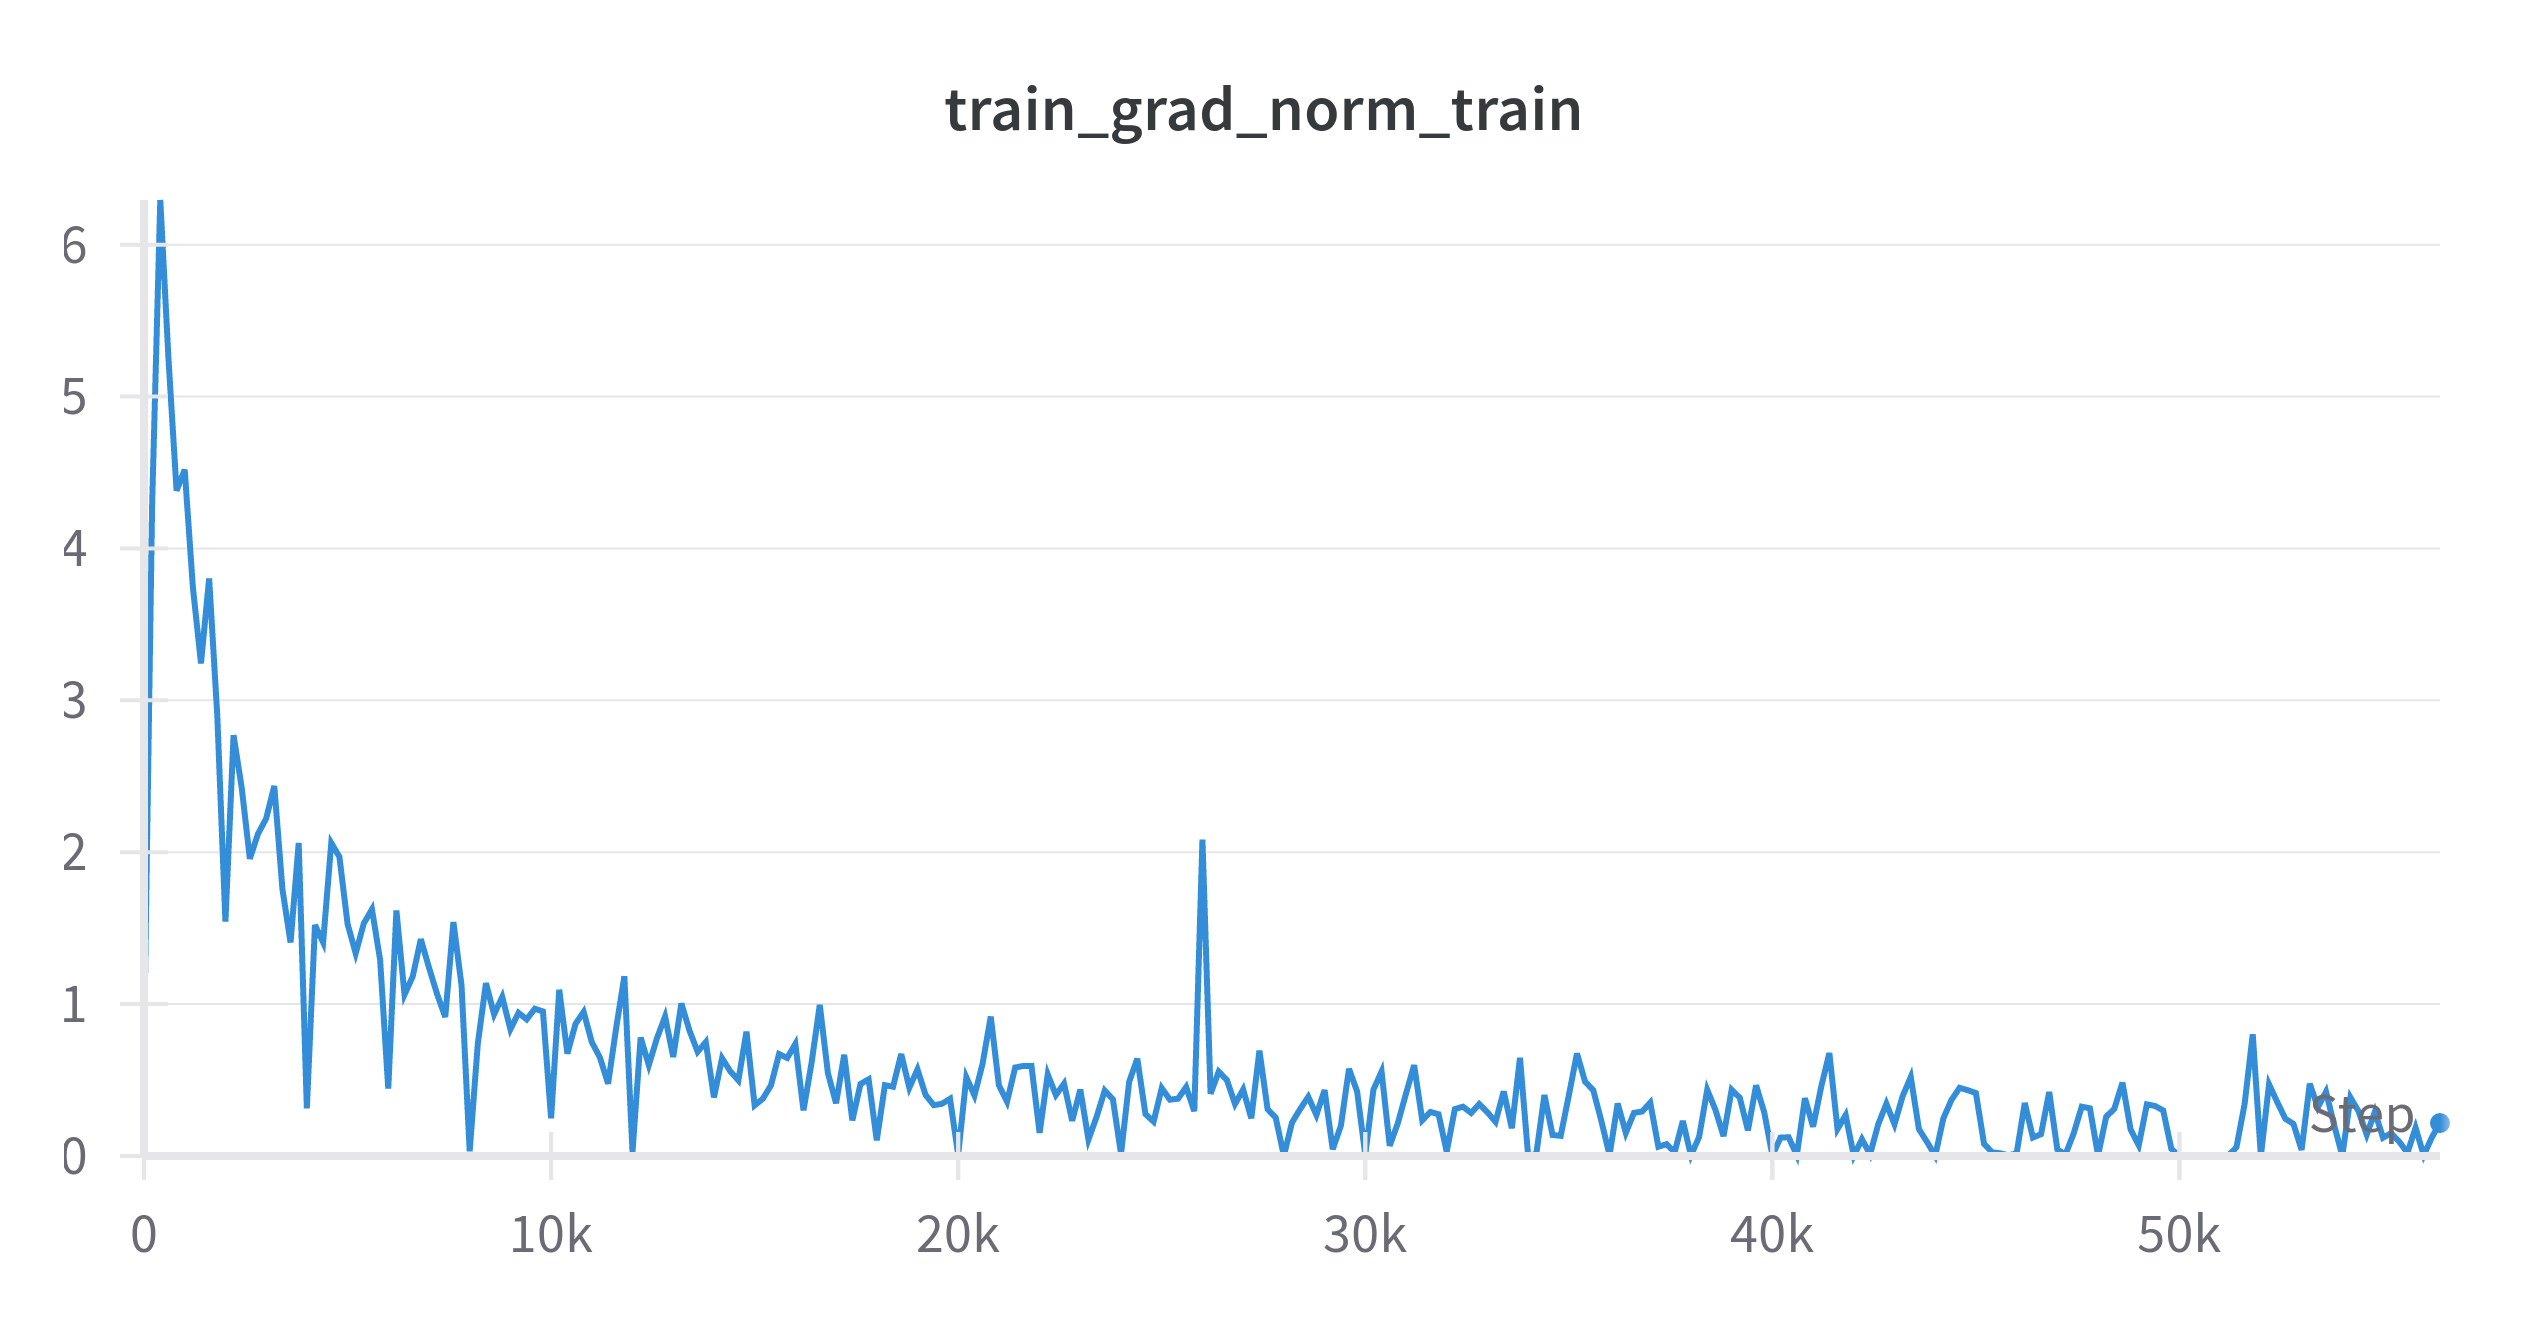
\includegraphics[width=400pt]{grad-norm.png} \end{center}



\section{Ablations}

\subsection{One GRU layer instead of three}

Link: \url{https://wandb.ai/elexunix/as_project/runs/8yv1t0zm?workspace=user-elexunix}.

Test EER score of the model: 0.07859.

It follows that the impact is noticeable, but not huge, and maybe long training can lead to the desired score, but I don't know. It seems a bit worse, though.

The paper doesn't mention the number of these GRU layers (I didn't notice).

\subsection{Remove weights from cross entropy}

More precisely, set them to 1. 1. instead of 1. 9.

Link: \url{https://wandb.ai/elexunix/as_project/runs/mcy64xah?workspace=user-elexunix}.

Test EER score of the model: 0.05096.

In fact, I expected this would matter more...

\subsection{Remove abs from the sinc layer}

Simply removing abs from from the formulas will not be anymore explainable that way, so it will probably not work good. Let's see.

Link: \url{https://wandb.ai/elexunix/as_project/runs/h7havmc4?workspace=user-elexunix}.

Test EER score of the model: 0.05740.

I was not right, it seems to work.

The paper doesn't comment on this matter.

\subsection{Zero weight decay}

This will of course lead to overfitting, even with our wd of $10^{-4}$ we have a strong one. The number of parameters is vastly more than the number of answers in the train part (the ratio is approximately 1000), training without huge regularization is strongly recommended against for your and your model's health.

Link: \url{https://wandb.ai/elexunix/as_project/runs/l98p8btf?workspace=user-elexunix}.

Test EER score of the model: 0.06581.

Actually, I thought it would be worse.

\subsection{Conv HPs as in the old paper}

Sinc filter length is already 1024.

Number of channels in this experiment is reduced from 128 to 20, from 512 to 128.

This is the recommendation from the old paper (but not the new one).

Link: \url{https://wandb.ai/elexunix/as_project/runs/n3xx0owb?workspace=user-elexunix}

Test EER score of the model: 0.10102.

This was obviously not trained for too long, it would be very long.

\subsection{Non-zero min\_low\_hz, min\_band\_hz}

In this setup, we try setting min\_low\_hz, min\_band\_hz both to 50. This will probably lead to poor processing of frequencies below approximately 50Hz, which is not that low and probably human voice has some reverbations in these ranges as well...

Link: \url{https://wandb.ai/elexunix/as_project/runs/9hev2bm3?workspace=user-elexunix}.

Test EER score of the model: 0.07884.

The paper doesn't discuss these values.

The results seem to agree with the prediction in this case.



\section{Another sinc layer type}

The sinc layer type used in the main run was S1 (equal spacing in Mels). I have also implemented S2 (equal spacing in Hertz)

Link for the test run: \url{https://wandb.ai/elexunix/as_project/runs/gch8vhg3?workspace=user-elexunix}.

Test EER score of the model (this was not trained for too long, as this is just a demonstration that it learns): 0.05766.



\section{Full description of new and modified code}

\subsection{hw\_code/collate\_fn/collate.py}

New function \texttt{as\_collate\_fn} has been defined. This function is used to collate fields in dataset items that have the same length. It takes in a list of dictionaries representing dataset items. It uses torch default collate.

\subsection{hw\_code/datasets/\_\_init\_\_.py}

Minor import changes.

\subsection{hw\_code/losses/\_\_init\_\_.py}

Minor import-related changes.

\subsection{hw\_code/model/\_\_init\_\_.py}

Import-related changes: new folders for each hw are created, and our folder is hw\_code/model/hw5as.

\subsection{hw\_code/utils/object\_loading.py}

Essentially, \verb|pin_memory=True| was added (may require more RAM, but may help with speed).

\subsection{hw\_code/utils/trainer/\_\_init\_\_.py}

Minor import-related changes.

\subsection{hw\_code/config/config.json}

Oh...

\subsubsection{Changes in top-level keys}

\begin{itemize}
    \item \texttt{sr}: The value of \texttt{sr} has been changed from 22050 to 16000.
\end{itemize}

\subsubsection{Changes in model configuration}

\begin{itemize}
    \item \texttt{type}: The value of \texttt{type} has been changed from \texttt{"HiFiGAN"} to \texttt{"RawNet2Model"}.
\end{itemize}

\subsubsection{Changes in model arguments}

\begin{itemize}
    \item \texttt{n\_mels}: The key \texttt{n\_mels} has been removed.
    \item \texttt{lrelu\_slope}: The key \texttt{lrelu\_slope} has been removed.
\end{itemize}

\subsubsection{Changes in training configuration}

\begin{itemize}
    \item \texttt{batch\_size}: The value of \texttt{batch\_size} has been changed from 16 to 32.
\end{itemize}

\subsubsection{Changes in training dataset configuration}

\begin{itemize}
    \item \texttt{type}: The value of \texttt{type} has been changed from \texttt{"LJSpeechDataset"} to \texttt{"ASVSpoofDataset"}.
    \item \texttt{segment\_size}: The value of \texttt{segment\_size} has been changed from 8192 to 64000.
\end{itemize}

\subsubsection{Changes in validation configuration}

\begin{itemize}
    \item \texttt{batch\_size}: The value of \texttt{batch\_size} has been changed from 16 to 256. Yes! It just works faster this way.
\end{itemize}

\subsubsection{Changes in validation dataset configuration}

\begin{itemize}
    \item \texttt{type}: The value of \texttt{type} has been changed from \texttt{"LJSpeechDataset"} to \texttt{"ASVSpoofDataset"}.
\end{itemize}

\subsubsection{Changes in test configuration}

\begin{itemize}
    \item \texttt{batch\_size}: The value of \texttt{batch\_size} has been changed to 256.
    \item \texttt{num\_workers}: The value of \texttt{num\_workers} has been changed from 0 to 0.
\end{itemize}

\subsubsection{Changes in test dataset configuration}

\begin{itemize}
    \item \texttt{type}: The value of \texttt{type} has been changed from \texttt{"LJSpeechDataset"} to \texttt{"ASVSpoofDataset"}.
\end{itemize}

\subsubsection{Changes in optimizer configuration}

\begin{itemize}
    \item \texttt{lr}: The value of \texttt{lr} has been changed from 3e-4 to 1e-4.
    \item \texttt{weight\_decay}: The value of \texttt{weight\_decay} has been changed to 1e-4.
\end{itemize}

\subsubsection{Changes in learning rate scheduler configuration}

\begin{itemize}
    \item \texttt{type}: The value of \texttt{type} has been changed from \texttt{"OneCycleLR"} to \texttt{"ExponentialLR"}.
    \item \texttt{gamma}: The value of \texttt{gamma} has been set to 1.
\end{itemize}

\subsubsection{Changes in trainer configuration}

\begin{itemize}
    \item \texttt{log\_interval}: The value of \texttt{log\_interval} has been changed from 50 to 200.
    \item \texttt{monitor}: The value of \texttt{monitor} has been changed from \texttt{"min val\_total\_loss"} to \texttt{"min valid\_loss"}.
\end{itemize}

\subsubsection{Changes in WandB configuration}

\begin{itemize}
    \item \texttt{wandb\_project}: The value of \texttt{wandb\_project} has been changed from \texttt{"nv\_project"} to \texttt{"as\_project"}.
    \item \texttt{len\_epoch}: The value of \texttt{len\_epoch} has been changed from 400 to 2000.
\end{itemize}

%\subsection{hw\_code/trainer/as\_trainer.py: new file based on nv\_trainer.py}
\subsection{ASTrainer class description}

It is actually easier to describe what is in the new trainer than how it differs from the previous one... There are really a lot of differences. So here the description of ASTrainer class goes:

The \texttt{ASTrainer} class is a subclass of the \texttt{BaseTrainer} class and is responsible for training the Anti-Spoofing model. Here is a detailed description of the class and its methods:

\subsubsection{Constructor (\_\_init\_\_)}

The constructor initializes the \texttt{ASTrainer} class with the following parameters:

\begin{itemize}
    \item \texttt{model}: The Anti-Spoofing model.
    \item \texttt{metrics}: The list of metrics to evaluate during training.
    \item \texttt{optimizer}: The optimizer for model parameter updates.
    \item \texttt{config}: The configuration dictionary.
    \item \texttt{device}: The device (CPU or GPU) to use for training.
    \item \texttt{dataloaders}: A dictionary of dataloaders for the training, validation, and test datasets.
    \item \texttt{lr\_scheduler}: The learning rate scheduler.
    \item \texttt{len\_epoch}: Length of an epoch (number of iterations). If not provided, the length of the training dataloader is used.
    \item \texttt{skip\_oom}: A boolean flag indicating whether to skip batches that result in out-of-memory errors.
\end{itemize}

\subsubsection{Helper Methods}

\begin{itemize}
    \item \texttt{move\_batch\_to\_device()}: Moves the batch data to the given device (CPU or GPU).
    \item \texttt{\_clip\_grad\_norm()}: Clips the gradient norm of the model parameters if \texttt{grad\_norm\_clip} is defined in the trainer configuration.
    \item \texttt{\_progress()}: Returns a formatted string showing the progress of the current epoch during training.
    \item \texttt{get\_grad\_norm()}: Calculates and returns the gradient norm of the model parameters.
\end{itemize}

\subsubsection{Training Methods}

\begin{itemize}
    \item \texttt{process\_batch()}: Processes a batch of data by moving it to the device, performing forward pass, calculating the loss, updating the metrics, and backpropagating the gradients if in training mode.
    \item \texttt{\_train\_epoch()}: The main training logic for an epoch. It iterates over the training dataloader, processes each batch, and updates the metrics. It also logs the train metrics and returns them as a log.
    \item \texttt{\_validation\_epoch()}: Performs the validation after training an epoch. It evaluates the model on the validation dataset, updates the validation metrics, and logs them.
    \item \texttt{\_test\_epoch()}: Performs the testing after training an epoch. It evaluates the model on the test dataset, updates the test metrics, and logs them. It also computes the Equal Error Rate (EER) using the \texttt{compute\_eer()} function.
\end{itemize}

\subsubsection{Training Process}

The training process follows these steps:

\begin{enumerate}
    \item The model is set to train mode, and the train metrics are reset.
    \item For each batch in the training dataloader:
    \begin{enumerate}
        \item The batch is processed using the \texttt{process\_batch()} method.
        \item The train metrics are updated.
        \item If the batch index is divisible by the log step, the train metrics are logged.
        \item If the batch index is greater than or equal to the length of the epoch, the training loop is exited.
    \end{enumerate}
    \item The validation and test epochs are run using the \texttt{\_validation\_epoch()} and \texttt{\_test\_epoch()} methods, respectively. The metrics from each of these epochs are added to the log.
    \item The log is returned, containing average loss and metrics for the epoch.
\end{enumerate}

This class provides a complete implementation of the training and evaluation process for the Anti-Spoofing model.

\subsection{ASVspoof Loss Function Description}

The ASVspoof loss function is defined in the file \texttt{hw\_code/losses/asvspoof\_losses.py}. Here is a description of the loss function:

\begin{itemize}
    \item \texttt{CE\_weights}: It is a tensor that contains the weights for the classes in the cross-entropy loss. In this case, the tensor contains the weights \texttt{[1., 9.]}, where the first class has weight 1 and the second class has weight 9. This tensor is stored on the CUDA device.
    \item \texttt{loss(predicted, target)}: This function calculates the cross-entropy loss between the predicted and target tensors. The \texttt{predicted} tensor represents the predicted class probabilities, and the \texttt{target} tensor represents the ground truth class labels. The loss is computed using the \texttt{F.cross\_entropy()} function from the \texttt{torch.nn.functional} module, with the weights \texttt{CE\_weights}. The calculated loss is returned.
\end{itemize}

The ASVspoof loss function computes the cross-entropy loss with weighted classes for a classification task, where the first class has a weight of 1 and the second class has a weight of 9. This weighted loss can help in handling class imbalance and assigning more importance to certain classes during training.

\subsection{ASVSpoofDataset Class Description}

The \texttt{ASVSpoofDataset} class represents the dataset for the ASVspoof challenge. Here is a detailed description of the class and its methods:

\subsubsection{Constructor (\_\_init\_\_)}

The constructor initializes the \texttt{ASVSpoofDataset} class with the following parameters:

\begin{itemize}
    \item \texttt{segment\_size}: The size of each audio segment to extract.
    \item \texttt{data\_dir}: The path to the directory containing the dataset. If not provided, the default path is used.
    \item \texttt{part}: Indicates the part of the dataset to load, i.e., "train", "valid", or "test".
    \item \texttt{max\_size}: The maximum number of samples to load from the dataset.
    \item \texttt{shuffle}: A boolean value indicating whether to shuffle the dataset.
    \item \texttt{*args, **kwargs}: Additional arguments that can be passed to the constructor.
\end{itemize}

\subsubsection{Methods}

\begin{itemize}
    \item \texttt{\_\_getitem\_\_(self, index)}: This method returns a sample from the dataset at the specified index. It loads the audio file using the \texttt{torchaudio.load()} function, retrieves the audio tensor, and trims it to the desired segment size. The trimmed audio tensor and the corresponding label are returned as a dictionary.

    \item \texttt{\_\_len\_\_(self)}: This method returns the length of the dataset, which is equal to the number of audio files available.
\end{itemize}

The \texttt{ASVSpoofDataset} class represents the ASVspoof dataset for the given part ("train", "valid", or "test"). It reads the audio files from the specified directory and provides access to the audio data and corresponding labels. During initialization, the dataset is checked to ensure that it contains the expected number of samples for the specified part.

The dataset is designed to work with audio files in FLAC format. The \texttt{torchaudio.load()} function is used to load the audio files, and the resulting audio tensors are processed to extract the desired segment size.

If a maximum size is specified, the dataset will be truncated to the specified number of samples. The dataset can also be shuffled during initialization by setting the \texttt{shuffle} parameter to \texttt{True}.

The dataset is designed to be used with PyTorch's \texttt{torch.utils.data} module, allowing for easy integration with data loaders and training pipelines. By accessing individual samples using the \texttt{\_\_getitem\_\_} method, training, validation, and testing procedures can be performed using this dataset.

\subsection{hw\_code/model/hw5as/\_\_init\_\_.py: empty file}

\subsection{SincConvEpic Class Description}

The \texttt{SincConvEpic} class represents the SincConvEpic module, which performs Sinc convolution on audio waveforms. Here is a more detailed description of the class and its methods, including the mathematical details:

\subsubsection{Constructor (\_\_init\_\_)}

The constructor initializes the \texttt{SincConvEpic} class with the following parameters:

\begin{itemize}
    \item \texttt{in\_channels}: The number of input channels in the audio waveforms. This should be 1 since audio typically has a single channel.
    \item \texttt{out\_channels}: The number of output channels (filters) in the Sinc convolution layer.
    \item \texttt{kernel\_size}: The size of the SincConv kernel.
    \item \texttt{sample\_rate}: The sample rate of the audio waveforms.
\end{itemize}

The constructor initializes the instance variables \texttt{out\_channels}, \texttt{kernel\_size}, \texttt{sample\_rate}, and \texttt{cnt} (which is half of the kernel size).

The frequency range of the Sinc filters is determined by the sample rate. The frequencies are equally spaced in the Mel scale between 0 and half of the sample rate. The frequencies are initialized as trainable parameters using \texttt{nn.Parameter}. The trainable frequencies are represented by two sets of parameters: \texttt{trainable\_f1s} and \texttt{trainable\_f2s}.

\subsubsection{Methods}

\begin{itemize}
    \item \texttt{forward(self, waveforms)}: This method performs the forward pass of the SincConvEpic module. It takes the input waveforms and applies the SincConv operation. The trainable Sinc filter frequencies (\texttt{trainable\_f1s} and \texttt{trainable\_f2s}) are used to compute the frequencies for each output channel. The sinc functions are computed by applying the hamming window to the sampled time. The band-pass filters are obtained by subtracting the sinc function of frequency 1 from the sinc function of frequency 2. Finally, the input waveforms are convolved with the band-pass filters using the \texttt{F.conv1d()} function. The resulting output is returned.
\end{itemize}

Additionally, the class defines the following static methods:

\begin{itemize}
    \item \texttt{hz\_to\_mel(hz)}: This method converts frequencies from Hertz (Hz) to the Mel scale. It uses the formula: \(\text{{Mel}} = 2595 \log_{10}(1 + \frac{{\text{{hz}}}}{{700}})\).
    \item \texttt{mel\_to\_hz(mel)}: This method converts frequencies from the Mel scale to Hertz (Hz). It uses the formula: \(\text{{Hz}} = 700 \left(10^{\frac{{\text{{mel}}}}{{2595}}} - 1\right)\).
\end{itemize}

The \texttt{SincConvEpic} class provides the functionality of applying Sinc convolution on audio waveforms. It allows for customization of the number of output channels, kernel size, and sample rate, making it suitable for various audio processing tasks.

The SincConv operation involves creating band-pass filters using sinc functions. The frequency range of the filters is determined by the trainable parameters. By using trainable frequencies, the SincConvEpic module can adapt to different input and output requirements.


\end{document}